 %\documentclass[xcolor=dvipsnames]{beamer}
 \documentclass[xcolor=dvipsnames,12pt]{beamer}
%\documentclass[xcolor=dvipsnames,11pt,handout]{beamer}
%\documentclass[xcolor=dvipsnames,12pt,handout]{beamer}

%\useoutertheme{infolines}

\usepackage{color}

%\usetheme{Madrid}

%\usecolortheme[named=OliveGreen]{structure}

\makeatletter
\colorlet{beamer@blendedblue}{orange!70!red}
\makeatother
%\usecolortheme{orchid}
%\usecolortheme{orange}

\setbeamertemplate{navigation symbols}{}

\usepackage{bbold, graphicx, latexsym, verbatim, amsmath, amssymb, amsthm, dsfont, tikz, mathtools, tipa, marvosym, graphics,datetime, import,pdfpages}

\usepackage [english]{babel}
\usepackage [autostyle, english = american]{csquotes}
\usepackage{grffile}
\MakeOuterQuote{"}



\newtheorem{thm}{Theorem}

\theoremstyle{definition}

\newtheorem*{defn}{Definition}
\DeclareMathOperator{\acc}{acc}
\DeclareMathOperator{\low}{L}
\DeclareMathOperator{\Prob}{P}
\DeclareMathOperator{\hi}{H}
\DeclareMathOperator{\wProb}{w/ probability}
\DeclareMathOperator{\Img}{Im}

\DeclareMathOperator{\LHS}{LHS}

\DeclareMathOperator{\RHS}{RHS}
\DeclareMathOperator{\centralized}{centralized}
\newcommand*{\proofbreak}{\usebeamertemplate{proof end}\framebreak\usebeamertemplate{proof begin}}

%\title[Strategic Customer Behavior, Commitment and Supply Chain Performance]{"Noisy Communication"\\ (QME 2007) \\by Bharat Anand and Ron Shacar (QME 2007)}

\title[Bundling]{ Bundling in Ecommerce\\ a Case Study of the DSLX Camera Market}


\author[Chen and Zhong]{Xin Chen and Zemin Zachary Zhong}

\institute[UC Berkeley - Haas]{University of California -- Berkeley}

\date{Mar. 30, 2016}
%\graphicspath {{figures/}}
\begin{document}
\begin{frame}
\titlepage
\end{frame}

%\begin{frame}
%\includegraphics[page=20,scale = 0.46]{ppt}
%\end{frame}

\begin{frame}{Preview}
	\begin{enumerate}
		\item Introduction to Taobao
		\item Motivation and Research Question
		\item Summary of Findings
		\begin{itemize}
		\item Bundle Price Distribution
		\item Method of Current Street Price Calibration
		\item Summary Statistics
		\item Reduced Form Results
		\end{itemize}
		\item Nitty-gritty of Data
	\end{enumerate}
\end{frame}

%fixme consec page arg
{\setbeamercolor{background canvas}{bg=}
\begin{center}

\includepdf[pages=2]{ppt20160329}
%Canon 700d pic
\includepdf[pages=6]{ppt20160329}
\includepdf[pages=59]{ppt20160329}
\includepdf[pages=60]{ppt20160329}
\end{center}
}

\begin{frame}{How many consumers buy Bundles?}
	\graphicspath{ {./graph_share/} }
	\centering
	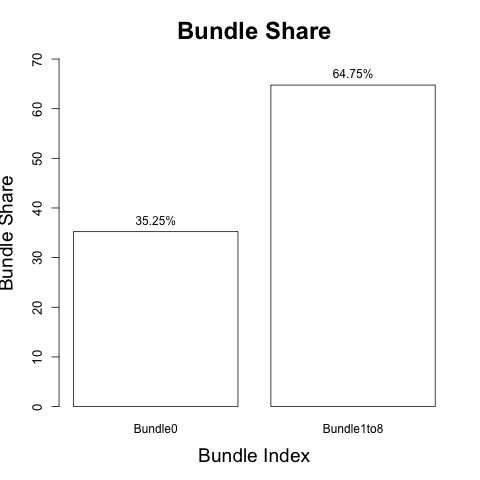
\includegraphics[scale=0.48]{Avg_Bundle_Share1}
\end{frame}

\begin{frame}{Average Bundle Share}
	\graphicspath{ {./graph_share/} }
	\centering
	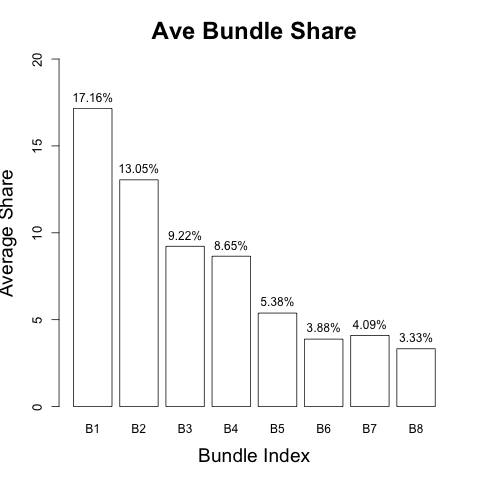
\includegraphics[scale=0.48]{Avg_Bundle_Share2}
\end{frame}

{\setbeamercolor{background canvas}{bg=}
\begin{center}
\includepdf[pages=3]{ppt20160329}
\includepdf[pages=4]{ppt20160329}
\includepdf[pages=5]{ppt20160329}
%Data page
%\includepdf[pages=7]{ppt20160329}
\end{center}
%%pages Selects pages to insert. The argument is a comma separated list,
%containing page numbers (pages={3,5,6,8}), ranges of page numbers
%(pages={4-9}) or any combination. To insert empty pages use {}.
%E.g.: pages={3,{},8-11,15} will insert page 3, an empty page, and
%pages 8, 9, 10, 11, and 15.
%1Actually not only links but all kinds of PDF annotations will get lost.
%2
%Page ranges are specied by the following syntax: hmi-hni. This selects
%all pages from hmi to hni. Omitting hmi defaults to the rst page; omit-
%ting hni defaults to the last page of the document. Another way to select
%the last page of the document, is to use the keyword last. (This is only
%permitted in a page range.)
%E.g.: pages=- will insert all pages of the document, and pages=last-1
%will insert all pages in reverse order.
%(Default: pages=1)
}

%fixme too many layers
\begin{frame}{Overview of Data}

\begin{enumerate}
\item Search Results Page 
\item View Item Page 
	\begin{itemize}
		\item	Structured Data
		\begin{itemize}
				\item	Number of Bundles and Pricing
				\item	Seller Reputation
%				\item	Aggregate Demand 
%					\begin{itemize}
					\item	Transaction Records (no longer available after Jan 25, 2016)
					\item	Cumulative Review as a proxy 
%					\end{itemize}
		\end{itemize}
		\item	Unstructured Data
				\begin{itemize}
					\item	Bundle Content
					\end{itemize}
	\end{itemize}
\end{enumerate}
\end{frame}

%graphs start here
\begin{frame}{Bundle Price}
\begin{figure}
%\includegraphics[scale=0.43]{1_histogram_of_deln}
%\scalebox{0.8}{
\graphicspath{ {../../0_relative_to_bundle_0/} }
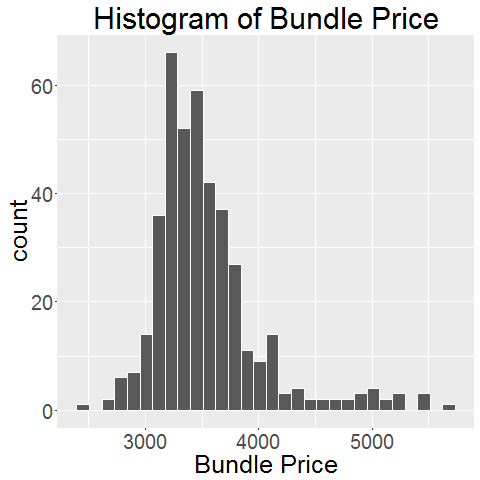
\includegraphics[scale=0.43]{7_z_histogram_bundle_price}
%}
\end{figure}
\end{frame}

\begin{frame}{Bundle Price}
\begin{figure}
%\includegraphics[scale=0.43]{1_histogram_of_deln}
%\scalebox{0.8}{
\graphicspath{ {../../0_relative_to_bundle_0/} }
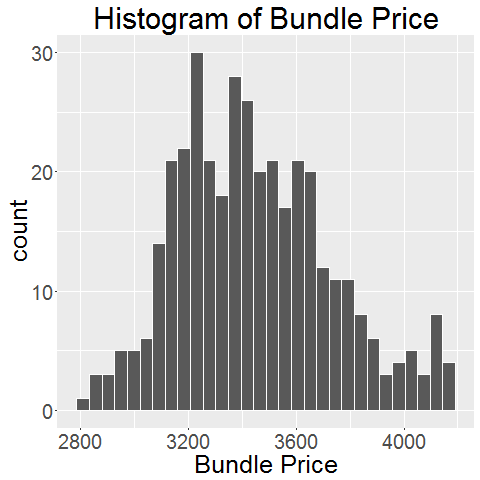
\includegraphics[scale=0.43]{7_zz_histogram_bundle_price_zoom_in}
%}
\end{figure}
\end{frame}

\begin{frame}{Bundle Price}
\begin{figure}
%\includegraphics[scale=0.43]{1_histogram_of_deln}
%\scalebox{0.8}{
\graphicspath{ {../../0_relative_to_bundle_0/} }
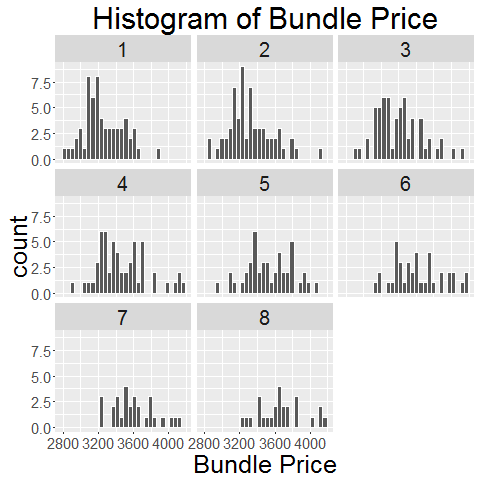
\includegraphics[scale=0.43]{7_zzz_histogram_bundle_price_in_different_bundle_index_zoom_in}
%}
\end{figure}
\end{frame}

\begin{frame}{Bundle Price}
\begin{figure}
%\includegraphics[scale=0.43]{1_histogram_of_deln}
%\scalebox{0.8}{
\graphicspath{ {../../0_relative_to_bundle_0/} }
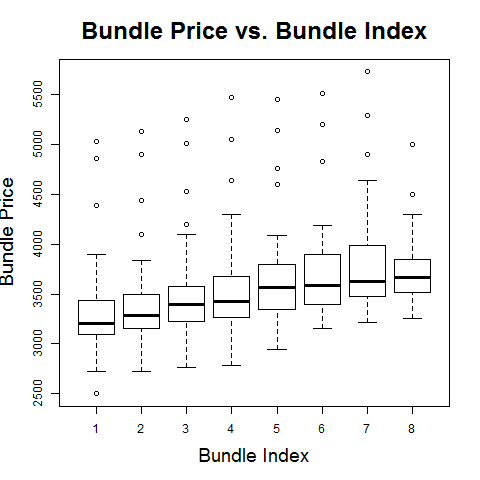
\includegraphics[scale=0.43]{7_zzzz_boxplot_bundle_price_bundle_index}
%}
\end{figure}
\end{frame}

%fixme bundle price v index zoomed in here

%formula

\begin{frame}{Definitions rel to $B_k$}
Notations
\begin{itemize}
	
	\item $p(B_j)$ - Bundle Price of Bundle $j$, $0 \le j \le 8$ 
	\item $p_{\acc}$ - Accessory Street Price \pause
	 	\begin{itemize}
	 		\item current reference price - mode price of all matching results on the first search result page
	 		%\item many different ways of defining it
	 	\end{itemize}
%	\item $\Delta p$ - Bundle Premium of $B_j$  rel to $B_k$% (k = 0, 1)$
%
%\pause
%%
%%
%
%$$\Delta p = p(B_j) - p(B_k) - \sum_{\forall \acc \in B_j \& \notin B_k} p(\acc)$$
%
%\item $\Delta n$ - \# of accessories in $B_j$ and not in $B_k$ 
\end{itemize}
\end{frame}

%example of equivalent of  \includepdf[pages=73-81], which does not work
{\setbeamercolor{background canvas}{bg=}

\begin{center}
%this part inserts the first slide
	\begin{tikzpicture}[remember picture, overlay]
	  \node at (current page.center) { \includegraphics[page=73,scale=0.505]{ppt20160329}};
	\end{tikzpicture}
%this part inserts the first slide

\includepdf[pages=74-81]{ppt20160329}
\end{center}


}


\begin{frame}{Definitions rel to $B_k$}
Notations
\begin{itemize}
	
	\item $p(B_j)$ - Bundle Price of Bundle $j$, $0 \le j \le 8$ 
	\item $p_{\acc}$ - Accessory Street Price
	 	\begin{itemize}
	 		\item current reference price - mode price of all matching results on the first search result page
	 		\item many different ways of defining it
	 	\end{itemize}  \pause
	\item $\Delta p$ - Bundle Premium of $B_j$  rel to $B_k$% (k = 0, 1)$

\pause
%
%

$$\Delta p = p(B_j) - p(B_k) - \sum_{\forall \acc \in B_j \& \notin B_k} p_{\acc}$$ \pause

\item $\Delta n$ - \# of accessories in $B_j$ and not in $B_k$ 

\end{itemize}
\end{frame}

\begin{frame}{Relative to Bundle 0}
\begin{figure}
%\includegraphics[scale=0.43]{1_histogram_of_deln}
%\scalebox{0.8}{
\graphicspath{ {../../0_relative_to_bundle_0/} }
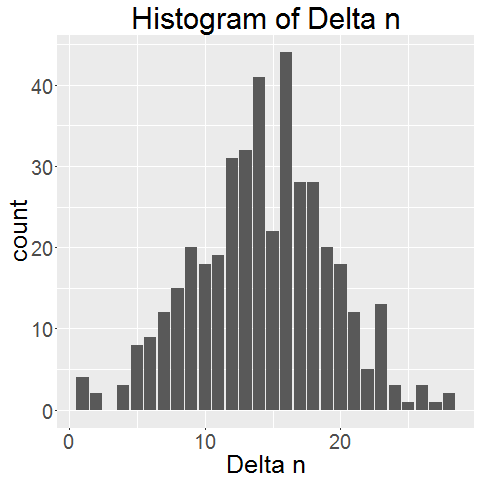
\includegraphics[scale=0.43]{1_histogram_of_delta_n_rel_to_b0}
%}
\end{figure}
\end{frame}

\begin{frame}{Relative to Bundle 0}
\begin{figure}
%\includegraphics[scale=0.43]{1_histogram_of_deln}
%\scalebox{0.8}{
\graphicspath{ {../../0_relative_to_bundle_0/} }
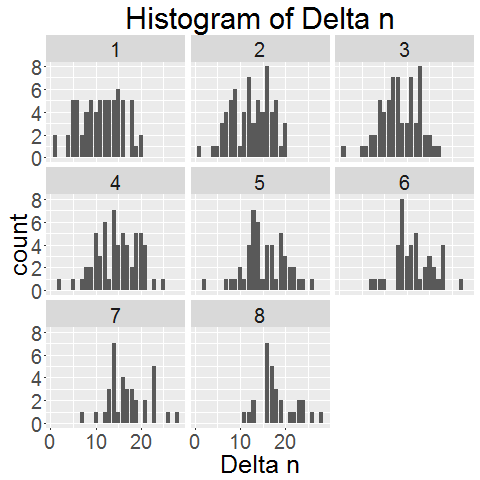
\includegraphics[scale=0.43]{1_z_histogram_of_delta_n_rel_to_b0_in_num_of_acc_relerent_bundle_index_rel_to_b0}
%}
\end{figure}
\end{frame}

\begin{frame}{Relative to Bundle 0}
\begin{figure}
%\includegraphics[scale=0.43]{1_histogram_of_deln}
%\scalebox{0.8}{
\graphicspath{ {../../0_relative_to_bundle_0/} }
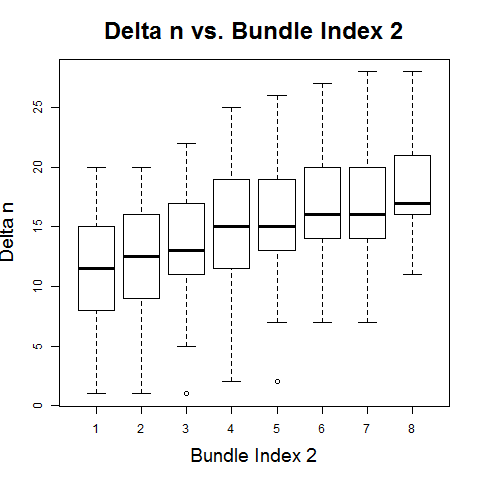
\includegraphics[scale=0.43]{2_boxplot_delta_n_bundle_index_rel_to_b0}
%}
\end{figure}
\end{frame}

\begin{frame}{Relative to Bundle 0}
\begin{figure}
%\includegraphics[scale=0.43]{1_histogram_of_deln}
%\scalebox{0.8}{
\graphicspath{ {../../0_relative_to_bundle_0/} }
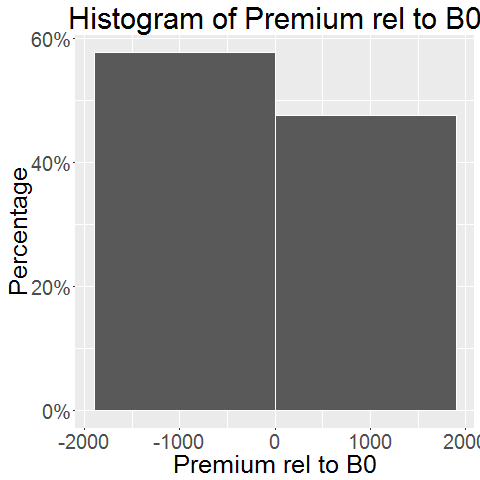
\includegraphics[scale=0.43]{3_histogram_of_prem_rel_to_b0_2_col}
%}
\end{figure}
\end{frame}

\begin{frame}{Relative to Bundle 0}
\begin{figure}
%\includegraphics[scale=0.43]{1_histogram_of_deln}
%\scalebox{0.8}{
\graphicspath{ {../../0_relative_to_bundle_0/} }
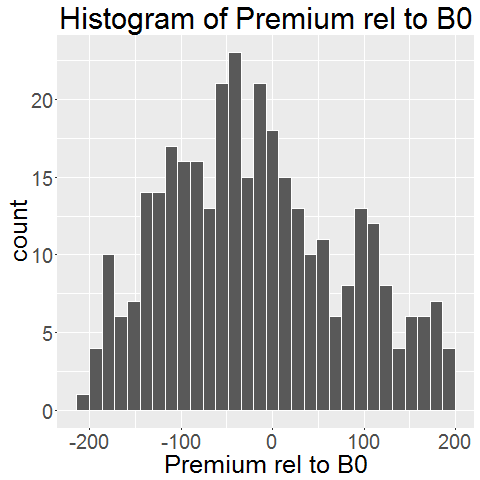
\includegraphics[scale=0.43]{5_histogram_of_prem_rel_to_b0_zoom_in_}
%}
\end{figure}
\centering
\textcolor{orange}{
{\Huge
Avg Premium $= 30$ RMB}
}
\end{frame}

\begin{frame}{Relative to Bundle 0}
\begin{figure}
%\includegraphics[scale=0.43]{1_histogram_of_deln}
%\scalebox{0.8}{
\graphicspath{ {../../0_relative_to_bundle_0/} }
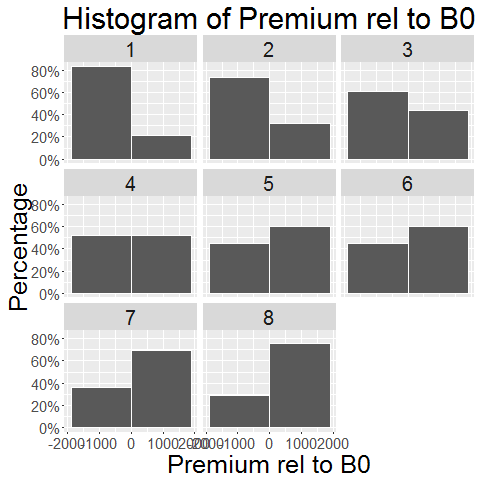
\includegraphics[scale=0.43]{3_z_histogram_of_prem_rel_to_b0_2_col_in_num_of_acc_relerent_bundle_index}
%}
\end{figure}
\end{frame}

\begin{frame}{Summary of Findings so far}
Relative to B0 Comparison
\begin{enumerate}
	\item $\approx 50\%$ of the Bundle Premium $\ge 0 $ \pause
	\item Avg Premium $= 30$ RMB \pause
	\item $> 50\%$ of the Bundle Premium $\ge 0 $ for Bundles 4-8\pause
	\item \% of Premium $\ge 0 \uparrow$ as Bundle Index $\uparrow$ \pause 
	\item Could it be the case that an even larger fraction have 
	\begin{center}
	Premium  $\ge 0 $  \pause
	\end{center}
	\item Potential Source of Bias: Huge Measurement Error in the Reference Acc Street Price \pause
	%\item Solution: Try a New Comparison Reference Bundle: 

%Bundle 1 instead of Bundle 0
\end{enumerate}
\end{frame}

{\setbeamercolor{background canvas}{bg=}
\begin{center}
\includepdf[pages=92]{ppt20160329}
\end{center}
}

%rel1 starts here
\begin{frame}{Relative to Bundle 1}
\begin{figure}
%\includegraphics[scale=0.43]{1_histogram_of_deln}

%\scalebox{0.8}{
\graphicspath{ {../../1_relative_to_bundle_1/} }
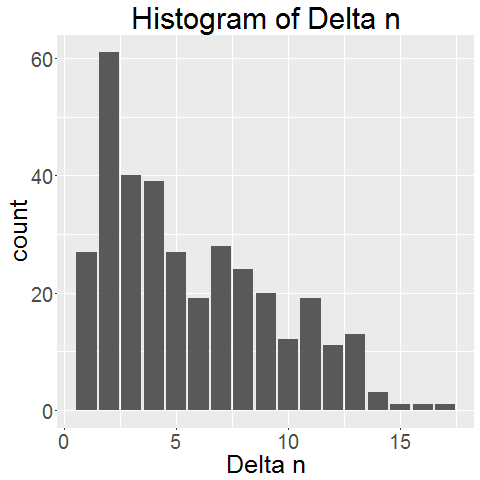
\includegraphics[scale=0.43]{1_histogram_of_delta_n_rel_to_bundle_1}
%}
\end{figure}
\end{frame}

%fixme
\begin{frame}{Relative to Bundle 1}
\begin{figure}
%\includegraphics[scale=0.43]{1_histogram_of_deln}

%\scalebox{0.8}{
\graphicspath{ {../../1_relative_to_bundle_1/} }
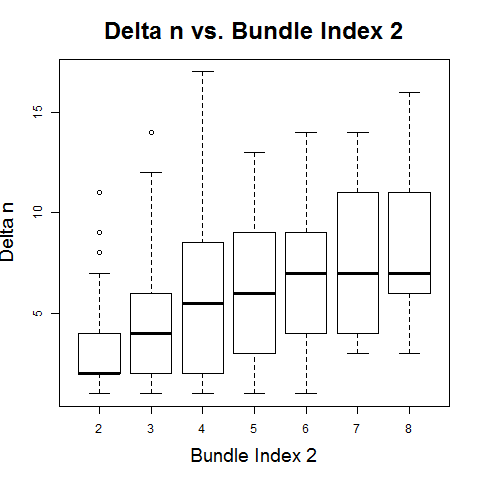
\includegraphics[scale=0.43]{2_boxplot_delta_n_bundle_index2_rel_to_bundle_1}
%}
\end{figure}
\end{frame}



\begin{frame}{Relative to Bundle 1}
\begin{figure}
%\includegraphics[scale=0.43]{1_histogram_of_deln}

%\scalebox{0.8}{
\graphicspath{ {../../1_relative_to_bundle_1/} }
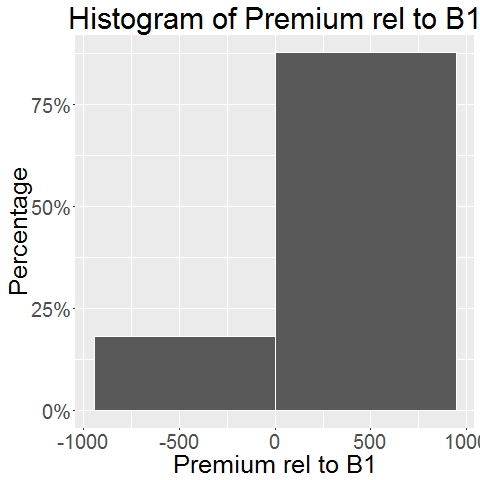
\includegraphics[scale=0.43]{3_histogram_of_prem_rel_to_bundle_1_2_col.png}
%}
\end{figure}
\end{frame}

\begin{frame}{Comparison of Premium}
\begin{figure}
%\includegraphics[scale=0.43]{1_histogram_of_deln}

%\scalebox{0.8}{
\graphicspath{ {../../0_relative_to_bundle_0/} }
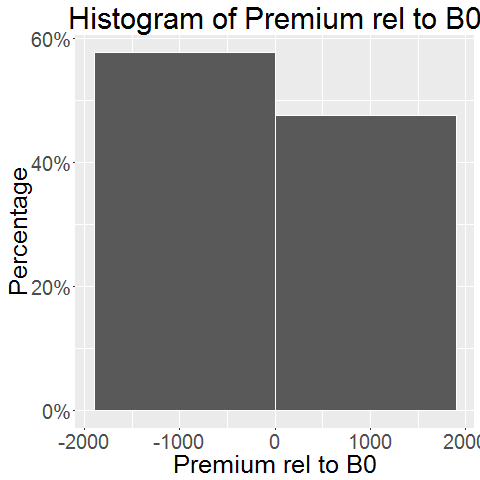
\includegraphics[width=0.475\textwidth]{3_histogram_of_prem_rel_to_b0_2_col}
\hfill
\graphicspath{ {../../1_relative_to_bundle_1/} }
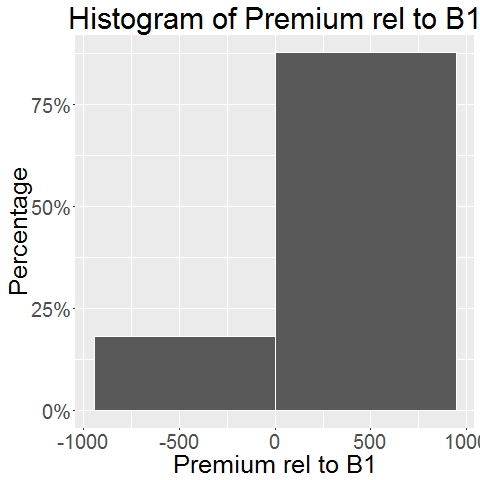
\includegraphics[width=0.475\textwidth]{3_histogram_of_prem_rel_to_bundle_1_2_col.png}
%}
\end{figure}
\end{frame}



\begin{frame}{Relative to Bundle 1}
\begin{figure}
%\includegraphics[scale=0.43]{1_histogram_of_deln}

%\scalebox{0.8}{
\graphicspath{ {../../1_relative_to_bundle_1/} }
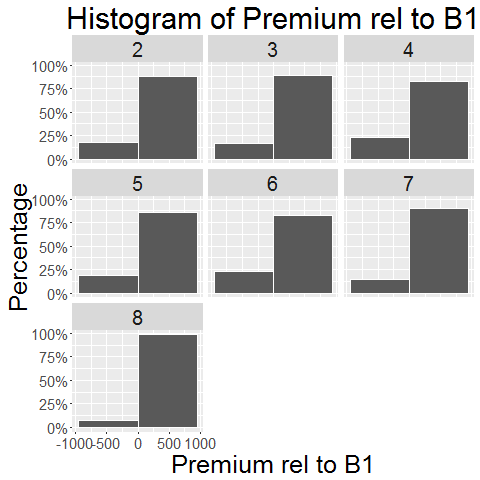
\includegraphics[scale=0.43]{3_z_histogram_of_prem_rel_to_bundle_1_2_col_in_different_bundle_index}
%}
\end{figure}
\end{frame}

\begin{frame}{Comparison of Premium}
\begin{figure}
%\includegraphics[scale=0.43]{1_histogram_of_deln}
\graphicspath{ {../../0_relative_to_bundle_0/} }
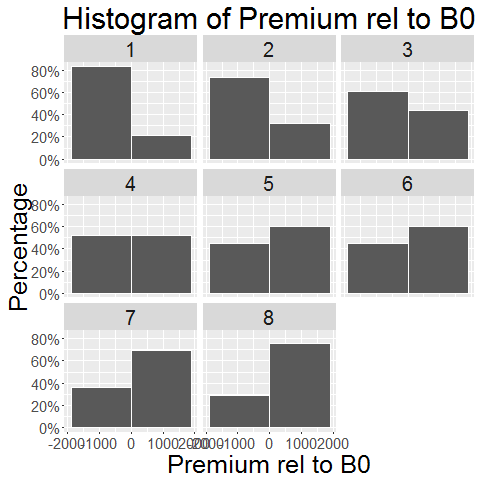
\includegraphics[width=0.475\textwidth]{3_z_histogram_of_prem_rel_to_b0_2_col_in_num_of_acc_relerent_bundle_index}
\hfill
%\scalebox{0.8}{
\graphicspath{ {../../1_relative_to_bundle_1/} }
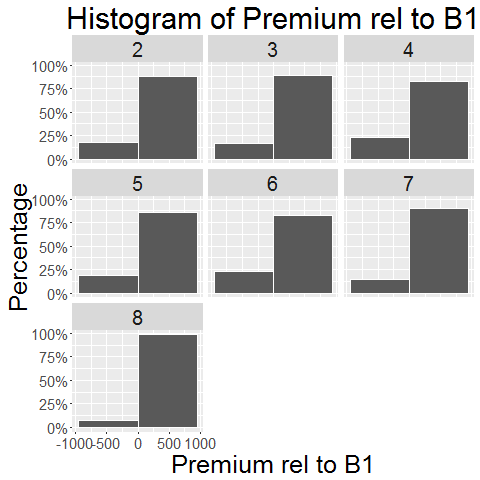
\includegraphics[width=0.475\textwidth]{3_z_histogram_of_prem_rel_to_bundle_1_2_col_in_different_bundle_index}
%}
\end{figure}
\end{frame}


\begin{frame}{Relative to Bundle 1}
\begin{figure}
%\includegraphics[scale=0.43]{1_histogram_of_deln}

%\scalebox{0.8}{
\graphicspath{ {../../1_relative_to_bundle_1/} }
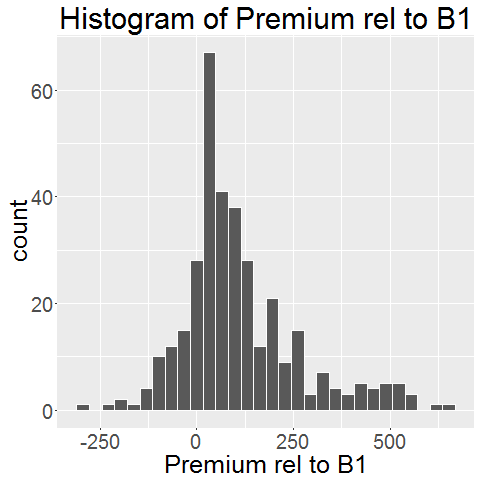
\includegraphics[scale=0.43]{4_histogram_of_prem_rel_to_bundle_1}
%}
\end{figure}
\end{frame}

\begin{frame}{Relative to Bundle 1}
\begin{figure}
%\includegraphics[scale=0.43]{1_histogram_of_deln}

%\scalebox{0.8}{
\graphicspath{ {../../1_relative_to_bundle_1/} }
\includegraphics[scale=0.43]{5_histogram_of_prem_rel_to_bundle_1_zoom_in_}
%}
\end{figure}
\begin{center}
\textcolor{orange}{{\Huge Avg Premium = $111$ RMB}} %110.69 
\end{center}
\end{frame}

\begin{frame}{Research Question and Modeling Assumptions}

Question: 

How does a seller decide on 
\begin{itemize} \item what to offer at each position (bundle\_index)?
 \item what bundle premium to charge ($\Delta p$)?
\end{itemize}
\medskip
%\pasue

Assumptions:
\begin{itemize}
	\item $B_1$ and price of $B_1$ are given exogenously
	\item a collection of bundles $\mathcal{B}$ are given exogenously %$\{B_j | 2 \le j \le 8 \}$ are given exogenously
	\item $\forall B \in \mathcal{B}$  $\Delta n $  rel $B_1$ is exogenously given %(for each $B_j$ w/ $2 \le j \le 8$) is exogenously given
	
%		\begin{itemize}
%			\item seller first sets the price of $B_1$
%			\item  market competition force a price of $B_1$
%		\end{itemize}
	\item $\forall B \in \mathcal{B}$ seller decides on the bundle position j %for each given bundle B
	\item $\forall B \in \mathcal{B}$ seller decides on the bundle premium $\Delta p$
\end{itemize}
\end{frame}

\begin{frame}{Relative to Bundle 1}
\begin{figure}
%\includegraphics[scale=0.43]{1_histogram_of_deln}

%\scalebox{0.8}{
\graphicspath{ {../../1_relative_to_bundle_1/} }
\includegraphics[width=0.475\textwidth]{6_boxplot_bundle_index_prem_rel_to_bundle_1}
\hfill
%%}
%\end{figure}
%\end{frame}
%
%\begin{frame}{Relative to Bundle 1}
%\begin{figure}
%%\includegraphics[scale=0.43]{1_histogram_of_deln}
%
%%\scalebox{0.8}{
%\graphicspath{ {../../1_relative_to_bundle_1/} }
\includegraphics[width=0.475\textwidth]{7_boxplot_delta_n_prem_rel_to_bundle_1}
%}
\end{figure}
\end{frame}

\begin{frame}{Regression}
\begin{align*} \Delta p = \alpha \Delta n + \beta \text{bundle\_index}\\ \pause
 +\gamma_1 \mathbb{1}(\text{memory card (cc)} \in \Delta n) \\
+ \gamma_2 \mathbb{1}(\text{uv filter (uv)} \in \Delta n) \\
+ \gamma_3  \mathbb{1}(\text{camera bag (bag)} \in \Delta n)
\end{align*}
\medskip
\pause

memory card, uv filter, and camera bags are the three accessory categories that appear most frequently in both 

$\Delta n$ rel $B_0$ and $\Delta n$ rel $B_1$
\end{frame}

\begin{frame}{Regression}
\centering
%Modification of First Attempt


\scalebox{0.7}{
\documentclass[]{article}
\setlength{\pdfpagewidth}{8.5in} \setlength{\pdfpageheight}{11in}
\begin{document}
\begin{tabular}{lcc} \hline
 & (1) & (2) \\
VARIABLES & premrel & premrel \\ \hline
 &  &  \\
diff & -13.41*** & -16.05*** \\
 & (4.347) & (5.318) \\
bundle\_index2 & 5.939*** & 6.290*** \\
 & (1.868) & (2.017) \\
ind\_cc & -1.354 & 3.377 \\
 & (17.03) & (18.61) \\
ind\_uv & 9.291 & 15.97 \\
 & (22.40) & (22.67) \\
ind\_xb &  & 34.11 \\
 &  & (28.51) \\
Constant & 57.28*** & 56.10*** \\
 & (17.75) & (18.37) \\
 &  &  \\
Observations & 352 & 352 \\
R-squared & 0.068 & 0.076 \\
 Number of item\_id & 67 & 67 \\ \hline
\multicolumn{3}{c}{ Robust standard errors in parentheses} \\
\multicolumn{3}{c}{ *** p$<$0.01, ** p$<$0.05, * p$<$0.1} \\
\end{tabular}
\end{document}

}\end{frame}

\begin{frame}{Results}
{\setbeamercolor{background canvas}{bg=}
\begin{center}

\includegraphics[page=94,scale = 0.46]{ppt20160329}

\end{center}
}
\end{frame}

\begin{frame}{Regression}

\centering
Verifying Assumption

\medskip

\scalebox{0.8}{
\documentclass[]{article}
\setlength{\pdfpagewidth}{8.5in} \setlength{\pdfpageheight}{11in}
\begin{document}
\begin{tabular}{lccc} \hline
 & (1) & (2) & (3) \\
VARIABLES & rel\_cost\_deln & rel\_cost\_deln & rel\_cost\_deln \\ \hline
 &  &  &  \\
diff & 38.64*** & 40.16*** & 41.15*** \\
 & (3.256) & (3.751) & (4.366) \\
ind\_cc & -57.34*** & -60.35*** & -61.61*** \\
 & (10.48) & (10.58) & (11.52) \\
ind\_uv &  & -42.51* & -43.52* \\
 &  & (25.07) & (25.61) \\
ind\_xb &  &  & -13.95 \\
 &  &  & (31.17) \\
Constant & -19.75 & -15.57 & -15.70 \\
 & (14.93) & (13.09) & (13.25) \\
 &  &  &  \\
Observations & 352 & 352 & 352 \\
R-squared & 0.669 & 0.675 & 0.675 \\
 Number of item\_id & 67 & 67 & 67 \\ \hline
\multicolumn{4}{c}{ Robust standard errors in parentheses} \\
\multicolumn{4}{c}{ *** p$<$0.01, ** p$<$0.05, * p$<$0.1} \\
\end{tabular}
\end{document}

}
\end{frame}

{\setbeamercolor{background canvas}{bg=}
\begin{center}
\includepdf[pages=93]{ppt20160329}
%Data page
%this part inserts the first slide
	\begin{tikzpicture}[remember picture, overlay]
	  \node at (current page.center) { \includegraphics[page=7,scale=0.505]{ppt20160329}};
	\end{tikzpicture}
%this part inserts the first slide
\includepdf[pages=8-80]{ppt20160329}
\end{center}
}






\end{document}